\section{Discussion \& Open Problems}\label{sec: discussion}

\body{Here we introduced tree co-width, a new graph invariant which is bounded on paths and trees, but also on some dense and symmetric classes of graphs, such as products of small graphs. The theory of tree co-width can be developed purely graph-theoretically. However, category theory provides conceptual guidance and structural insights that allow us to connect decomposition methods to stratified models in applications such as epidemiology, and design efficient algorithms that leverage universal properties. In particular, the category-theoretic treatment turns out to be essential, at least to the authors, in showing that first-order model checking can be performed directly on tree co-decompositions, without constructing their limits, in FPT-time parameterized by the width and the formula (with linear dependence on the number of bags).} 

\subsubsection{Relationships to Feferman-Vaught}

\body{
    It is worth comparing our results to general Feferman-Vaught results. For this we turn to Hodges' textbook~\cite{Hodges_1993} (specifically Equations 6.3, 6.4 and Theorem 9.6.2) where a general Feferman-Vaught theorem is given in terms of certain substructures of products $\prod_{i \in I}A_i$ called $B$-valued substructure, where $B$ is a Boolean algebra whose points are certain subsets of the index set $I$. At first glance, being substructures of products, these may seem similar to pullbacks, but they are in fact not. To see this, first observe that, if  $C\subseteq A_1\times A_2$ is a substructure and let $I=\{1,2\}$, then there are precisely two Boolean algebras of subsets of $I$: $B_1=\{\varnothing,I\}$ and $B_2= 2^I$. Thus $C$ admits gluing over $B_2$ if and only if $C=\pi_{A_1}(C)\times\pi_{A_2}(C)$ (this is already remarked by Hodges~\cite{Hodges_1993}). Furthermore, $C$ is $B_1$-valued if and only if $C \cong A_1 \cong A_2$.  Consequently, arbitrary pullbacks $A_1\times_A A_2$ need not satisfy Hodges' gluing and valuedness conditions for any Boolean algebra on $I$. To make this very concrete, consider any pair of surjections $X\twoheadrightarrow 2\twoheadleftarrow Y$ of sets: their pullback can satisfy Hodges' conditions only in the degenerate case where both maps are bijections.
}

\body{
    What the previous discussion \textit{does} establish is that our \cref{thm: FO model checking on codecompositions} does not follow \textit{verbatim} from what Hodges calls `{generalized Feferman-Vaught}'. However, it doesn't rule out the possibility of first hacking the structure -- by taking FO-interpretations or transductions, say -- and \textit{then} applying known results. Also, perhaps more interestingly, meta-theorems of the kind discussed above are somewhat hazy, as Hodges points out~\cite{Hodges_1993}, in the sense that many different kinds of results get lumped together under the umbrella term `Feferman-Vaught'. This presents a difficulty in evaluating where and how our result fits into that literature and indeed we cannot rule out the possibility obtaining an alternative proof of our algorithmic meta-theorems by leveraging some other kind of Feferman-Vaught-like result.
}

\body{
    Either way, there are some structural differences between typical proof techniques in this area and those we employed here. Whereas typical model-theoretic arguments rely on accounting for logical types, we explicitly manipulate proof-relevant data (meaning strategies and hypotheticals) in our dynamic programming arguments. These may be two sides of the same coin: just as interpretations allow us to reason either by transforming structures or by translating formulas in the opposite direction, preserving  satisfaction~\cite[Proposition 3.5]{immerman2012descriptive}, there may be a similar correspondence between composing logical types and composing the structures that witness their satisfaction. Earnestly engaging with these complexities and providing a more unified treatment of these techniques would be an interesting research program. It is, however, beyond the scope of the present paper. 
}


\begin{comment}
\subsubsection{Graphs of bounded co-width and FO tractable graph classes}



\begin{definition}[As defined in~\cite{GroheKreutzerSiebertz2017}]\label{def:nowhere-dense}
    For an integer $r\geq 0$, a graph $H$ is a \define{depth-$r$ minor} of a graph $G$ if there exist pairwise vertex-disjoint connected subgraphs $\{B_v\}_{v\in V(H)}$ of $G$, each having radius at most $r$ measured within that subgraph, such that every edge $uv\in E(H)$ is witnessed by an edge of $G$ joining a vertex of $B_u$ to a vertex of $B_v$. A graph class $\mathcal{C}$ is \define{nowhere dense} if, for every integer $r\geq 0$, there exists a finite graph $H_r$ such that $H_r$ is not a depth-$r$ minor of any graph in $\mathcal{C}$.
\end{definition}

\begin{definition}\label{def:monadically-stable}
    For each integer $n\geq 1$, the \define{half-graph} $H_n$ is the bipartite graph with parts $\{x_1,\ldots,x_n\}$ and $\{y_1,\ldots,y_n\}$ in which $x_i y_j$ is an edge if and only if $i\leq j$. A graph class $\mathcal{C}$ is \define{monadically stable} if no fixed FO transduction produces all half-graphs from $\mathcal{C}$. Equivalently, for every FO transduction $T$, there exists an integer $n\geq 1$ such that no graph in $T(\mathcal{C})$ is isomorphic to $H_n$, where $T(\mathcal{C})=\bigcup_{G\in\mathcal{C}}T(G)$.
\end{definition}

\begin{proposition}\label{prop:cow-not-structurally-nowhere-dense}
    There exists a class of graphs admitting path co-decompositions of width at most $4$ that is not structurally nowhere dense. In particular, bounded tree co-width does not imply structural nowhere denseness nor monadic stability.
\end{proposition}

\begin{proof}
    Let $B$ be the bipartite graph with vertex set $V(B)=\{\ell_0,\ell_1,r_0,r_1\}$ and edge set $E(B)=\{\ell_0r_0,\ell_0r_1,\ell_1r_0\}$, so that $B\cong P_4$. Writing $V(K_2)=\{a,b\}$, define the epimorphism $p:B \mapsto K_2$ by $p(\ell_0)=p(\ell_1)=a$ and $p(r_0)=p(r_1)=b$. 

    For each $n\geq 1$, let $\mathcal{T}_n$ be the path co-decomposition whose auxiliary path has $n$ nodes, whose bags are copies $B^{(1)},\ldots,B^{(n)}$ of $B$, whose adhesions are copies of $K_2$, and whose incidence maps are the corresponding copies of $p$. Let $D_n=\lim\mathcal{T}_n$ and $\mathcal{D}=\{D_n:n\geq 1\}$. Every bag has four vertices, so every graph in $\mathcal{D}$ admits a path co-decomposition of width $4$.

    A vertex of $D_n$ is a tuple $(v_1,\ldots,v_n)$ satisfying $p(v_1)=\cdots=p(v_n)$. Thus either all coordinates are either $\ell_i$ or $r_j$ vertices. For each binary string $\mathbf{a}=(a_1,\ldots,a_n)\in\{0,1\}^n$, write $L_{\mathbf{a}}=(\ell_{a_1}^{(1)},\ldots,\ell_{a_n}^{(n)})$ and $R_{\mathbf{a}}=(r_{a_1}^{(1)},\ldots,r_{a_n}^{(n)})$. These form the two parts of $D_n$. Adjacency holds coordinate-wise. As $\ell^{(t)}_1r^{(t)}_1$ are the only missing edges between the parts of $B$, we have that $L_{\mathbf{a}}R_{\mathbf{b}}\in E(D_n)$ if and only if $a_t b_t=0$ for every $t\in\{1,\ldots,n\}$. As there are no edges within either part of $B$, $D_n$ is bipartite.

    Let $H_n$ be the half-graph with bipartition $\{x_1,\ldots,x_n\}$ and $\{y_1,\ldots,y_n\}$, where $x_i y_j\in E(H_n)$ if and only if $i\leq j$. For each $i$, let $\mathbf{e}_i$ be the binary string whose only nonzero coordinate is coordinate $i$, and for each $j$, let $\mathbf{b}^{(j)}=0^j1^{n-j}$. In $D_n$, choose $x_i=L_{\mathbf{e}_i}$ and $y_j=R_{\mathbf{b}^{(j)}}$. Then $x_i y_j\in E(D_n)$ if and only if $b^{(j)}_i=0$, which holds precisely when $i\leq j$. The chosen vertices are pairwise distinct, and there are no edges among the $x_i$ or among the $y_j$. They therefore induce a copy of $H_n$.

    Every structurally nowhere dense class is monadically stable, and a monadically stable class cannot FO-transduce all half-graphs; see \cite[Section~3.3]{DreierMaehlmannSiebertz2023}. However, the fixed FO transduction defined by $\nu(x):=P(x)$ and $\eta(x,y):=E(x,y)$, where $P$ is an additional unary predicate, selects the subgraph induced by the vertices marked by $P$. For every $n$, marking the vertices of the induced copy of $H_n$ constructed above produces $H_n$ from $D_n$. Hence $\mathcal{D}$ FO-transduces all half-graphs and is not monadically stable. It follows that $\mathcal{D}$ is not structurally nowhere dense.
\end{proof}
\end{comment}

\subsection{Future Directions}
\body{Tree co-decompositions appear to be a rich topic which already straddles a few different research areas such as graph theory, finite model theory, category theory (as developed in this paper) and other areas including scientific modeling (albeit, framed in a different language; c.f. Libkind et al.~\cite{LibkindEtAl2022Epidemic}) and applied topology (under the guise of cellular shaves; c.f. Curry~\cite{Curry2014}, Hansen and Ghrist~\cite{HansenGhrist2019}, Robinson~\cite{Robinson2017} and Ribeiro, Ten{\'o}rio, Belieni Souza and Mesquita~\cite{ribeiro2026cooperative}). Given this range, it no surprise that further questions abound. Below we highlight several conjectures and open research directions that stem from the current paper and which suit the interests of the authors; this is by no means an exhaustive list.}

\paragraph{Some Questions in Graph Theory}

\body{
    Despite being closely related to tree-width by virtue of categorical duality, tree co-decompositions provide a notion of width that is genuinely distinct from tree-width. Moreover, classes of bounded co-width are distinct from those of bounded twin-width: as shown earlier, there are classes of graphs, such as powers of irreflexive complete graphs, which have bounded tree co-width but unbounded twin-width. The converse direction, however, is unclear.
}

\begin{question}
    Are there classes of bounded twin-width that have unbounded tree co-width?
\end{question}

\body{Although it can be shown that binary trees have bounded path co-width (in contrast to what happens when considering classical path-width), it is not clear whether all trees have bounded path co-width. Our characterization of bounded path co-width in terms of graph grammars (c.f. Apendix~\ref{appendix: grammar}) may provide an approach to this question. We believe that this class may be a candidate for separating path co-width from tree co-width asymptotically.}

\begin{conjecture}
    Trees -- even allowing loops -- have unbounded path co-width.
\end{conjecture}

\body{Although all categorical limits commute with each other, it is still interesting to investigate how tree co-width interacts with other algebraic graph operations.}
\begin{question}
    What can be said about the tree co-width of prime graphs (those not admitting nontrivial factorizations along categorical products)? Furthermore, can the tree co-width of a box-product of graphs be determined from the tree co-width of its factors?
\end{question}

\body{The uniqueness and canonicity of decompositions is another compelling direction. For instance, in \cref{fig:distinct}, we see genuinely different co-decompositions which build the same graph.
}

\begin{figure}
    \centering
    \includegraphics[width=0.5\linewidth, page=16]{LLJ-figs.pdf}
    \caption{Two genuinely distinct co-decompositions (left) which build the same graph (right).}
    \label{fig:distinct}
\end{figure} 

\body{
It is natural to ask whether there are canonical decompositions into prime pieces, for example an algebraic dual to the Tutte decomposition by Cunningham and Edmonds~\cite{CunninghamEdmonds1980}.}
\begin{question}
    Is there a canonical way to decompose graphs into prime pieces using tree co-decompositions with adhesions of size at most two?
\end{question}

\body{Co-decompositions of graphs pose some unique challenges when compared to classical graph decompositions. Some very intuitive properties of graph decompositions no longer hold in the dual setting. For example, given a pair of graphs $H$ and $G$ and a graph homomorphism $f \colon H\rightarrow G$, we have that any tree decomposition of $G$ can be `pulled back' along $f$ to a tree decomposition of $H$~\cite{BumpusKocsis2023}. More precisely, given a tree decomposition $(T,\{B_t\})$ of $G$, one can define a graph decomposition $(T,\{C_t\})$ of $H$ by setting each of the bags $C_t$ equal to the preimage $f^{-1}(B_t)$ of the bag $B_t$ in $H$. Importantly, the shape of the graph decomposition is preserved. And when $f$ is an inclusion, we get that the size of each bag decreases or stays the same: in other words, tree-width is subgraph monotone. One can view the preimage $f^{-1}(B_t)$ as the categorical pullback of the inclusion $B_t\hookrightarrow G$ and $f$.}

\body{In the classical setting, one can go further. In~\cite{bumpus2024pushing}, Bumpus, Fairbanks and Turner introduced \emph{lassos}, categorical structures which give rise to generalizations of graph contraction maps, and showed that tree-shaped structured decompositions can always be pushed forward along lasso-induced contractions, without increasing their width or changing their shape. In particular, this generalizes the familiar monotonicity of tree-width under graph contractions to a broad categorical setting. However, the arguments rely on the colimit structure of ordinary decompositions, and do not directly extend to co-decompositions, where the underlying object is instead reconstructed as a limit.}

\body{Indeed, it is natural to ask whether the machinery dualises: what happens when we push a co-decomposition forward along a graph homomorphism? Unfortunately, even the most direct construction fails. Pushing the constituent objects of a co-decomposition forward along a homomorphism does not, in general, produce a co-decomposition of the target object, as illustrated in~\autoref{fig:cant_copullback_codecomps}.
\begin{figure}
    \centering
    \begin{tikzpicture}[scale=0.7]
	\begin{pgfonlayer}{nodelayer}
		\node [style=black dot] (9) at (11, 1.5) {};
		\node [style=black dot] (10) at (9.5, 0) {};
		\node [style=black dot] (11) at (11, -1.5) {};
		\node [style=black dot] (12) at (12.5, 0) {};
		\node [style=black dot] (13) at (7.5, 2) {};
		\node [style=black dot] (14) at (9, 3.5) {};
		\node [style=black dot] (15) at (7.5, -2) {};
		\node [style=black dot] (16) at (7.5, -2) {};
		\node [style=black dot] (17) at (9, -3.5) {};
		\node [style=none] (18) at (8.75, 2.25) {};
		\node [style=none] (19) at (9, 2) {};
		\node [style=none] (20) at (9.75, 1.25) {};
		\node [style=none] (21) at (8.75, -2.25) {};
		\node [style=none] (22) at (9, -2) {};
		\node [style=none] (23) at (9.75, -1.25) {};
		\node [style=none] (24) at (8.75, -2) {};
		\node [style=none] (25) at (9, -1.75) {};
		\node [style=none] (26) at (9, -2.25) {};
		\node [style=none] (27) at (9.25, -2) {};
		\node [style=none] (28) at (8.75, 2) {};
		\node [style=none] (29) at (9, 2.25) {};
		\node [style=none] (30) at (9, 1.75) {};
		\node [style=none] (31) at (9.25, 2) {};
		\node [style=black dot] (32) at (20.75, 1.5) {};
		\node [style=black dot] (33) at (19.25, 0) {};
		\node [style=black dot] (35) at (22.25, 0) {};
		\node [style=black dot] (36) at (18, 3) {};
		\node [style=black dot] (39) at (18, -3) {};
		\node [style=none] (41) at (18.5, 2.25) {};
		\node [style=none] (42) at (18.75, 2) {};
		\node [style=none] (43) at (19.5, 1.25) {};
		\node [style=none] (44) at (18.5, -2.25) {};
		\node [style=none] (45) at (18.75, -2) {};
		\node [style=none] (46) at (19.5, -1.25) {};
		\node [style=none] (47) at (18.5, -2) {};
		\node [style=none] (48) at (18.75, -1.75) {};
		\node [style=none] (49) at (18.75, -2.25) {};
		\node [style=none] (50) at (19, -2) {};
		\node [style=none] (51) at (18.5, 2) {};
		\node [style=none] (52) at (18.75, 2.25) {};
		\node [style=none] (53) at (18.75, 1.75) {};
		\node [style=none] (54) at (19, 2) {};
		\node [style=none] (55) at (14.5, 0) {};
		\node [style=none] (56) at (18.25, 0) {};
		\node [style=none] (58) at (18, -0.25) {};
		\node [style=none] (59) at (18, 0.25) {};
		\node [style=none] (60) at (18, 0) {};
		\node [style=none] (61) at (17.75, 0.25) {};
		\node [style=none] (62) at (17.75, -0.25) {};
		\node [style=none] (63) at (10.5, 3) {};
		\node [style=none] (64) at (16.5, 3) {};
		\node [style=none] (65) at (16.25, 2.75) {};
		\node [style=none] (66) at (16.25, 3.25) {};
		\node [style=none] (67) at (16.25, 3) {};
		\node [style=none] (68) at (16, 3.25) {};
		\node [style=none] (69) at (16, 2.75) {};
		\node [style=none] (70) at (10.5, -3) {};
		\node [style=none] (71) at (16.5, -3) {};
		\node [style=none] (72) at (16.25, -3.25) {};
		\node [style=none] (73) at (16.25, -2.75) {};
		\node [style=none] (74) at (16.25, -3) {};
		\node [style=none] (75) at (16, -2.75) {};
		\node [style=none] (76) at (16, -3.25) {};
		\node [style=none] (77) at (7, 2.5) {$a$};
		\node [style=none] (78) at (8.5, 4) {$b$};
		\node [style=none] (79) at (7, -2.5) {$c$};
		\node [style=none] (80) at (8.5, -4) {$d$};
		\node [style=none] (81) at (8.5, 0) {$ac$};
		\node [style=none] (82) at (11, 2.5) {$bc$};
		\node [style=none] (83) at (13.5, 0) {$bd$};
		\node [style=none] (84) at (11, -2.5) {$ad$};
		\node [style=none] (85) at (22, 2.5) {$f(bc)=f(ad)$};
		\node [style=none] (86) at (19.25, -0.75) {$f(ac)$};
		\node [style=none] (87) at (22.25, -0.75) {$f(bd)$};
		\node [style=none] (88) at (16.25, 0.5) {$f$};
		\node [style=none] (89) at (16.75, 2) {};
		\node [style=none] (90) at (16.75, 1.5) {};
		\node [style=none] (91) at (17.25, 1.5) {};
		\node [style=none] (92) at (17.25, -1.5) {};
		\node [style=none] (93) at (16.75, -1.5) {};
		\node [style=none] (94) at (16.75, -2) {};
		\node [style=none] (95) at (12.5, -1.5) {$G$};
		\node [style=none] (96) at (20.75, -1) {$H$};
		\node [style=none] (97) at (7.25, 3.75) {$P$};
		\node [style=none] (98) at (7.25, -3.75) {$Q$};
	\end{pgfonlayer}
	\begin{pgfonlayer}{edgelayer}
		\draw [style=c0] (14) to (13);
		\draw [style=c0] (10) to (9);
		\draw [style=c0] (9) to (12);
		\draw [style=c0] (12) to (11);
		\draw [style=c0] (11) to (10);
		\draw [style=c0] (10) to (12);
		\draw [style=c0] (9) to (11);
		\draw [style=c0] (17) to (16);
		\draw [style=c0, in=90, out=0, loop] (14) to ();
		\draw [style=c0, in=-180, out=-90, loop] (13) to ();
		\draw [style=c0, in=-180, out=90, loop] (16) to ();
		\draw [style=c0, in=-90, out=0, loop] (17) to ();
		\draw [style=c0, in=-135, out=135, loop] (10) to ();
		\draw [style=c0, in=135, out=45, loop] (9) to ();
		\draw [style=c0, in=-45, out=45, loop] (12) to ();
		\draw [style=c0, in=-45, out=-135, loop] (11) to ();
		\draw [style=c0] (20.center) to (18.center);
		\draw [style=c0] (18.center) to (28.center);
		\draw [style=c0] (18.center) to (29.center);
		\draw [style=c0] (30.center) to (19.center);
		\draw [style=c0] (19.center) to (31.center);
		\draw [style=c0] (21.center) to (24.center);
		\draw [style=c0] (21.center) to (26.center);
		\draw [style=c0] (21.center) to (23.center);
		\draw [style=c0] (25.center) to (22.center);
		\draw [style=c0] (22.center) to (27.center);
		\draw [style=c0] (33) to (32);
		\draw [style=c0] (32) to (35);
		\draw [style=c0] (33) to (35);
		\draw [style=c0, in=45, out=135, loop] (36) to ();
		\draw [style=c0, in=45, out=135, loop] (39) to ();
		\draw [style=c0, in=-135, out=135, loop] (33) to ();
		\draw [style=c0, in=135, out=45, loop] (32) to ();
		\draw [style=c0, in=-45, out=45, loop] (35) to ();
		\draw [style=c0] (43.center) to (41.center);
		\draw [style=c0] (41.center) to (51.center);
		\draw [style=c0] (41.center) to (52.center);
		\draw [style=c0] (53.center) to (42.center);
		\draw [style=c0] (42.center) to (54.center);
		\draw [style=c0] (44.center) to (47.center);
		\draw [style=c0] (44.center) to (49.center);
		\draw [style=c0] (44.center) to (46.center);
		\draw [style=c0] (48.center) to (45.center);
		\draw [style=c0] (45.center) to (50.center);
		\draw [style=c0] (55.center) to (56.center);
		\draw [style=c0] (56.center) to (59.center);
		\draw [style=c0] (56.center) to (58.center);
		\draw [style=c0] (62.center) to (60.center);
		\draw [style=c0] (60.center) to (61.center);
		\draw [style=c0] (63.center) to (64.center);
		\draw [style=c0] (64.center) to (66.center);
		\draw [style=c0] (64.center) to (65.center);
		\draw [style=c0] (69.center) to (67.center);
		\draw [style=c0] (67.center) to (68.center);
		\draw [style=c0] (70.center) to (71.center);
		\draw [style=c0] (71.center) to (73.center);
		\draw [style=c0] (71.center) to (72.center);
		\draw [style=c0] (76.center) to (74.center);
		\draw [style=c0] (74.center) to (75.center);
		\draw [style=c0] (89.center) to (90.center);
		\draw [style=c0] (90.center) to (91.center);
		\draw [style=c0] (92.center) to (93.center);
		\draw [style=c0] (93.center) to (94.center);
	\end{pgfonlayer}
\end{tikzpicture}

    \caption{The graph $A$ is obtained from the graphs $P$ and $Q$ by pullback over the terminal graph $o$. Illustrated is the epimorphism $f:A\twoheadrightarrow B$ and the respective componentwise pushouts of the factors of $A$. The resulting diagram does not have $B$ as its pullback.}
    \label{fig:cant_copullback_codecomps}
\end{figure}
}

\body{Nevertheless, this does not rule out the existence of a more suitable class of morphisms under which co-decompositions behave well. Just as graph minors provide a natural containment relation with respect to which tree-width is monotone, it is reasonable to seek an analogous theory for tree co-width. Such a theory might also provide new tools for understanding obstructions to bounded co-width.}
\begin{question}
    Is there a natural analogue of graph minors for which tree co-width is monotone? More strongly, is there a class of morphisms along which tree co-decompositions can be pushed forward without increasing their width or changing their shape?
\end{question}

\paragraph{Some Questions in Algorithmics}

\body{Although it has not been our focus here, computing tree co-decompositions is an important task. In our motivating example in the introduction, Letícia built a stratified-model by specifying a co-decomposition. This means that the co-decomposition \textit{is} the input, while the larger model, the limit of the co-decomposition, is not (also because it can be huge! -- Letícia wouldn't want to write this down). However, from a purely graph-theoretic and algorithmic perspective, it is natural to ask how to compute a co-decomposition from an explicitly given graph. To that end, the computational complexity of determining co-width is largely unexplored; we conjecture it to be hard:}
\begin{conjecture}
    It is NP-hard to decide if a graph has tree co-width at most $k$.
\end{conjecture}

\body{Then again, factoring integers represented in unitary can be done in polynomial time and the same is true for factoring graphs as products~\cite{handbookproductgraphs}, so perhaps the conjecture above might fail. Either way, from a parameterized perspective, we expect it to be possible to efficiently compute minimum-width co-decompositions.}

\begin{conjecture}
    Deciding whether a graph has path (respectively, tree) co-width at most $k$ is in FPT parameterized by path (resp., tree) co-width.
\end{conjecture}

\begin{question}
    Which natural graph problems beyond first-order logic admit FPT algorithms parameterized by tree co-width when a co-decomposition is given? In particular, for which problems can hardness be established already at bounded tree co-width?
\end{question}

\body{Our algorithmic results also suggest several natural extensions. Perhaps the most immediate is counting first-order logic: rather than merely deciding whether a first-order formula is satisfied, can we count the number of assignments satisfying it? We expect that our methods can be extended to address this problem, with appropriate modifications to the dynamic programming tables. The main difficulty is to ensure that a satisfying assignment is counted exactly once, even when it admits multiple witnesses or strategies.}

\begin{conjecture}
    There is an algorithm which, given a tree co-decomposition $\mathcal T$ of width at most $w$ with $b$ bags, and a first-order formula $\phi(\bar x)$, computes
    \[
        \left|\left\{
            \bar a \mid
            \lim\mathcal T \models \phi(\bar a)
        \right\}\right|
    \]
    using $f_\sigma(w,|\phi|)\cdot b$ arithmetic operations, for some computable function $f_\sigma$ depending on the signature.
\end{conjecture}

\body{A related direction is extending our model-checking results to first-order logic with counting quantifiers, or to weighted variants of first-order logic. More broadly, one may ask how far the strategy-based methods developed here extend to other logics. The hardness of \textsc{Path} on implicitly represented graphs suggests that the boundary between tractability and intractability deserves particular attention, although it does not by itself rule out fixed-parameter tractability for more expressive logics.}
\begin{question}
    Which extensions of first-order logic admit fixed-parameter tractable model-checking algorithms on tree co-decompositions?
\end{question}

\paragraph{Categorical connections.}
\body{The construction of strategies and hypotheticals also suggests connections with other categorical approaches to logic. In particular, our use of families carrying explicit witnesses of logical compatibility is reminiscent of proof-relevant logical relations and Artin gluing, as developed, for example, by Sterling and Spitters~\cite{SterlingSpitters2018} and Sterling and Harper~\cite{SterlingHarper2021}. It would be interesting to investigate whether the categories of hypotheticals constructed here admit a natural description in terms of gluing or descent, and whether this perspective yields further algorithmic insights.}

\body{
    Our results also belong to the broader tradition of Feferman--Vaught--Mostowski composition methods. Recent categorical approaches, particularly the game-comonadic work of Jakl, Marsden and Shah~\cite{JaklMarsdenShah2022,JaklMarsdenShah2025}, provide general frameworks for logical composition and its algorithmic applications. An interesting direction is to clarify the relationship between these methods and our computation of supported hypotheticals over pullback-based tree co-decompositions.
    }

\body{
    Finally, consider contravariant powerset construction. Applying this construction to the constituent sets of a co-decomposition yields diagrams of Boolean algebras with compatibility maps running in the opposite direction -- specifically, these are structured decompositions~\cite{StructuredDecompositions} of Boolean Algebras. Taking colimits of these diagrams in categories of partial Boolean algebras, as studied by van den Berg and Heunen~\cite{vanDenBergHeunen2012} and Abramsky and Barbosa~\cite{AbramskyBarbosa2021} and building upon the work of Kochen and Specker~\cite{kochen2011problem}, suggests a possible connection with contextuality and the theory of partial algebras. Understanding this connection more precisely, and whether our algorithmic methods might find applications in that setting, seems a promising direction for future work.
}



\section*{Acknowledgements}

We thank \textit{Fábio Botler} for helpful discussions, \textit{Zoltan Kocsis} for pointing out the connection between our constructions and Artin gluing and for making us aware of categorical accounts of partial Boolean algebras, \textit{Johannes Carmesin} for pointing us towards comparisons with twin-width and \textit{Vinicius Fernandes dos Santos} for motivating us to establish the relationship between tree-width and co-width. 

Benjamin Merlin Bumpus acknowledges support of the \textit{São Paulo Research Foundation (FAPESP), grant 2025/16921-5}. Laura Larios-Jones acknowledges support of the \textit{University of Glasgow Jim Gatheral Travel Scholarship}. Will J.\ Turner acknowledges support by \textit{DFG project number 546892829}.

\section*{AI Methodology}
We used OpenAI's ChatGPT to assist with technical details and occasionally exposition of proofs, specifically when when drafting notation and wrangling index bookkeeping. AI use was also helpful for the construction of figures and illustrative examples; literature review; and brainstorming organizational options for the manuscript. We also used it as an effective sounding board for discussing and searching for counterexamples to conjectures and proposed arguments. All mathematical results and proof strategies were developed by the authors, who, of course, take full responsibility for the contents of the paper. The writing is also our own -- all em-dashes, of which the authors are fond of, were typed by hand. 
